% Options for packages loaded elsewhere
\PassOptionsToPackage{unicode}{hyperref}
\PassOptionsToPackage{hyphens}{url}
%
\documentclass[
]{article}
\usepackage{amsmath,amssymb}
\usepackage{lmodern}
\usepackage{iftex}
\ifPDFTeX
  \usepackage[T1]{fontenc}
  \usepackage[utf8]{inputenc}
  \usepackage{textcomp} % provide euro and other symbols
\else % if luatex or xetex
  \usepackage{unicode-math}
  \defaultfontfeatures{Scale=MatchLowercase}
  \defaultfontfeatures[\rmfamily]{Ligatures=TeX,Scale=1}
\fi
% Use upquote if available, for straight quotes in verbatim environments
\IfFileExists{upquote.sty}{\usepackage{upquote}}{}
\IfFileExists{microtype.sty}{% use microtype if available
  \usepackage[]{microtype}
  \UseMicrotypeSet[protrusion]{basicmath} % disable protrusion for tt fonts
}{}
\makeatletter
\@ifundefined{KOMAClassName}{% if non-KOMA class
  \IfFileExists{parskip.sty}{%
    \usepackage{parskip}
  }{% else
    \setlength{\parindent}{0pt}
    \setlength{\parskip}{6pt plus 2pt minus 1pt}}
}{% if KOMA class
  \KOMAoptions{parskip=half}}
\makeatother
\usepackage{xcolor}
\usepackage[margin=1in]{geometry}
\usepackage{color}
\usepackage{fancyvrb}
\newcommand{\VerbBar}{|}
\newcommand{\VERB}{\Verb[commandchars=\\\{\}]}
\DefineVerbatimEnvironment{Highlighting}{Verbatim}{commandchars=\\\{\}}
% Add ',fontsize=\small' for more characters per line
\usepackage{framed}
\definecolor{shadecolor}{RGB}{248,248,248}
\newenvironment{Shaded}{\begin{snugshade}}{\end{snugshade}}
\newcommand{\AlertTok}[1]{\textcolor[rgb]{0.94,0.16,0.16}{#1}}
\newcommand{\AnnotationTok}[1]{\textcolor[rgb]{0.56,0.35,0.01}{\textbf{\textit{#1}}}}
\newcommand{\AttributeTok}[1]{\textcolor[rgb]{0.77,0.63,0.00}{#1}}
\newcommand{\BaseNTok}[1]{\textcolor[rgb]{0.00,0.00,0.81}{#1}}
\newcommand{\BuiltInTok}[1]{#1}
\newcommand{\CharTok}[1]{\textcolor[rgb]{0.31,0.60,0.02}{#1}}
\newcommand{\CommentTok}[1]{\textcolor[rgb]{0.56,0.35,0.01}{\textit{#1}}}
\newcommand{\CommentVarTok}[1]{\textcolor[rgb]{0.56,0.35,0.01}{\textbf{\textit{#1}}}}
\newcommand{\ConstantTok}[1]{\textcolor[rgb]{0.00,0.00,0.00}{#1}}
\newcommand{\ControlFlowTok}[1]{\textcolor[rgb]{0.13,0.29,0.53}{\textbf{#1}}}
\newcommand{\DataTypeTok}[1]{\textcolor[rgb]{0.13,0.29,0.53}{#1}}
\newcommand{\DecValTok}[1]{\textcolor[rgb]{0.00,0.00,0.81}{#1}}
\newcommand{\DocumentationTok}[1]{\textcolor[rgb]{0.56,0.35,0.01}{\textbf{\textit{#1}}}}
\newcommand{\ErrorTok}[1]{\textcolor[rgb]{0.64,0.00,0.00}{\textbf{#1}}}
\newcommand{\ExtensionTok}[1]{#1}
\newcommand{\FloatTok}[1]{\textcolor[rgb]{0.00,0.00,0.81}{#1}}
\newcommand{\FunctionTok}[1]{\textcolor[rgb]{0.00,0.00,0.00}{#1}}
\newcommand{\ImportTok}[1]{#1}
\newcommand{\InformationTok}[1]{\textcolor[rgb]{0.56,0.35,0.01}{\textbf{\textit{#1}}}}
\newcommand{\KeywordTok}[1]{\textcolor[rgb]{0.13,0.29,0.53}{\textbf{#1}}}
\newcommand{\NormalTok}[1]{#1}
\newcommand{\OperatorTok}[1]{\textcolor[rgb]{0.81,0.36,0.00}{\textbf{#1}}}
\newcommand{\OtherTok}[1]{\textcolor[rgb]{0.56,0.35,0.01}{#1}}
\newcommand{\PreprocessorTok}[1]{\textcolor[rgb]{0.56,0.35,0.01}{\textit{#1}}}
\newcommand{\RegionMarkerTok}[1]{#1}
\newcommand{\SpecialCharTok}[1]{\textcolor[rgb]{0.00,0.00,0.00}{#1}}
\newcommand{\SpecialStringTok}[1]{\textcolor[rgb]{0.31,0.60,0.02}{#1}}
\newcommand{\StringTok}[1]{\textcolor[rgb]{0.31,0.60,0.02}{#1}}
\newcommand{\VariableTok}[1]{\textcolor[rgb]{0.00,0.00,0.00}{#1}}
\newcommand{\VerbatimStringTok}[1]{\textcolor[rgb]{0.31,0.60,0.02}{#1}}
\newcommand{\WarningTok}[1]{\textcolor[rgb]{0.56,0.35,0.01}{\textbf{\textit{#1}}}}
\usepackage{graphicx}
\makeatletter
\def\maxwidth{\ifdim\Gin@nat@width>\linewidth\linewidth\else\Gin@nat@width\fi}
\def\maxheight{\ifdim\Gin@nat@height>\textheight\textheight\else\Gin@nat@height\fi}
\makeatother
% Scale images if necessary, so that they will not overflow the page
% margins by default, and it is still possible to overwrite the defaults
% using explicit options in \includegraphics[width, height, ...]{}
\setkeys{Gin}{width=\maxwidth,height=\maxheight,keepaspectratio}
% Set default figure placement to htbp
\makeatletter
\def\fps@figure{htbp}
\makeatother
\setlength{\emergencystretch}{3em} % prevent overfull lines
\providecommand{\tightlist}{%
  \setlength{\itemsep}{0pt}\setlength{\parskip}{0pt}}
\setcounter{secnumdepth}{-\maxdimen} % remove section numbering
\ifLuaTeX
  \usepackage{selnolig}  % disable illegal ligatures
\fi
\IfFileExists{bookmark.sty}{\usepackage{bookmark}}{\usepackage{hyperref}}
\IfFileExists{xurl.sty}{\usepackage{xurl}}{} % add URL line breaks if available
\urlstyle{same} % disable monospaced font for URLs
\hypersetup{
  pdftitle={Analyse des accidents de la route pendant l'année 2021 en fonction du lieu, de la période, de l'age et du sexe},
  hidelinks,
  pdfcreator={LaTeX via pandoc}}

\title{Analyse des accidents de la route pendant l'année 2021 en
fonction du lieu, de la période, de l'age et du sexe}
\author{}
\date{\vspace{-2.5em}}

\begin{document}
\maketitle

{
\setcounter{tocdepth}{2}
\tableofcontents
}
\hypertarget{alex-delagrange-luxe9o-bouvier-lucas-giry-farah-seifeddine}{%
\subparagraph{Alex Delagrange, Léo Bouvier, Lucas Giry, Farah
Seifeddine}\label{alex-delagrange-luxe9o-bouvier-lucas-giry-farah-seifeddine}}

Dans ce rapport, nous cherchons à expliquer la gravité des accidents en
France en 2021

\hypertarget{etude-globale-sur-les-accidents-en-2021-en-france}{%
\subsection{Etude globale sur les accidents en 2021 en
France}\label{etude-globale-sur-les-accidents-en-2021-en-france}}

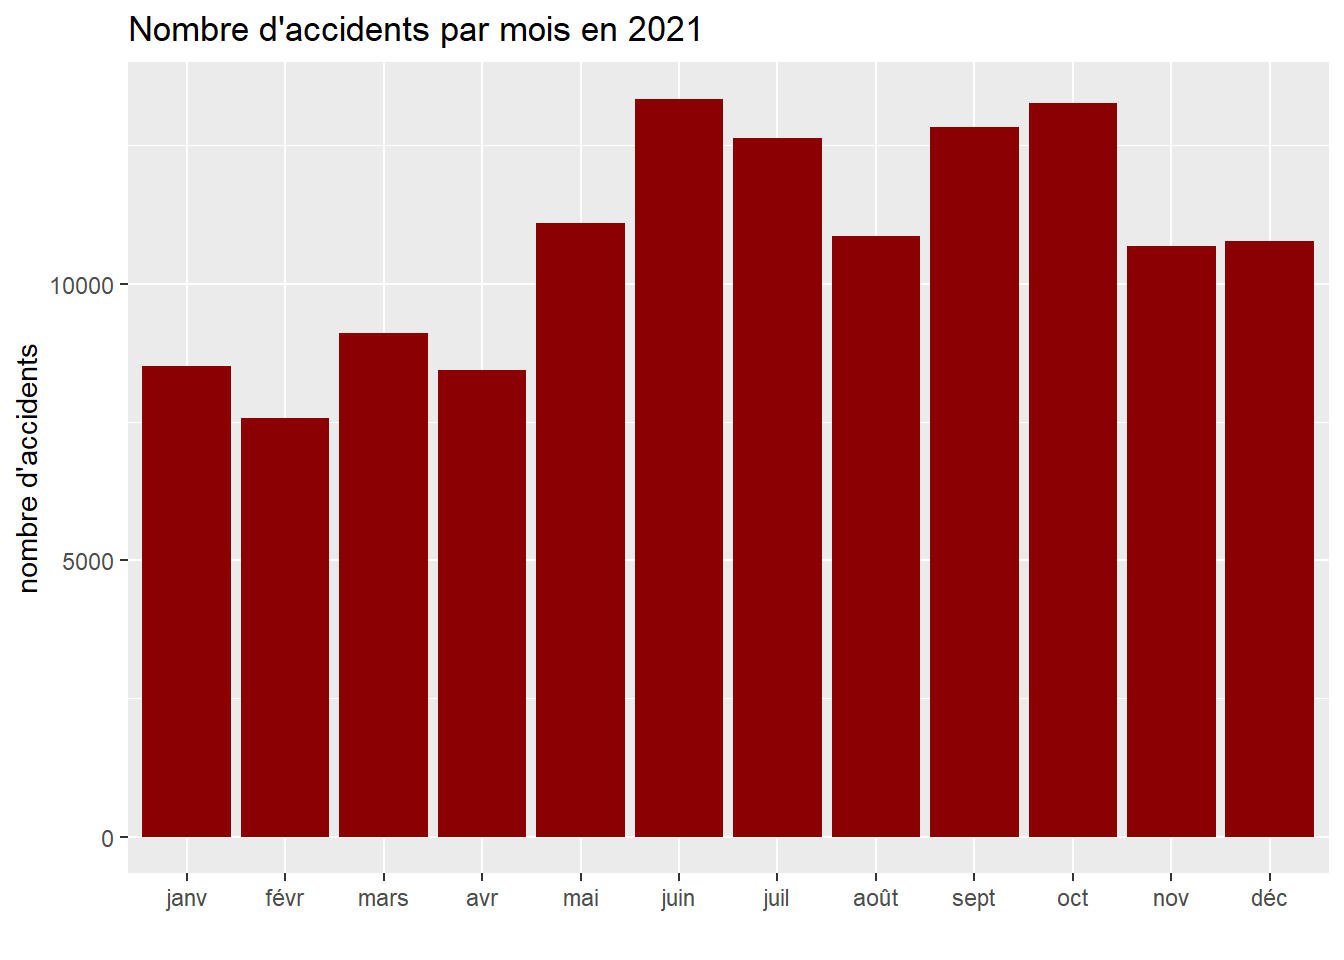
\includegraphics{FLAL_stats_files/figure-latex/pressure-1.pdf}

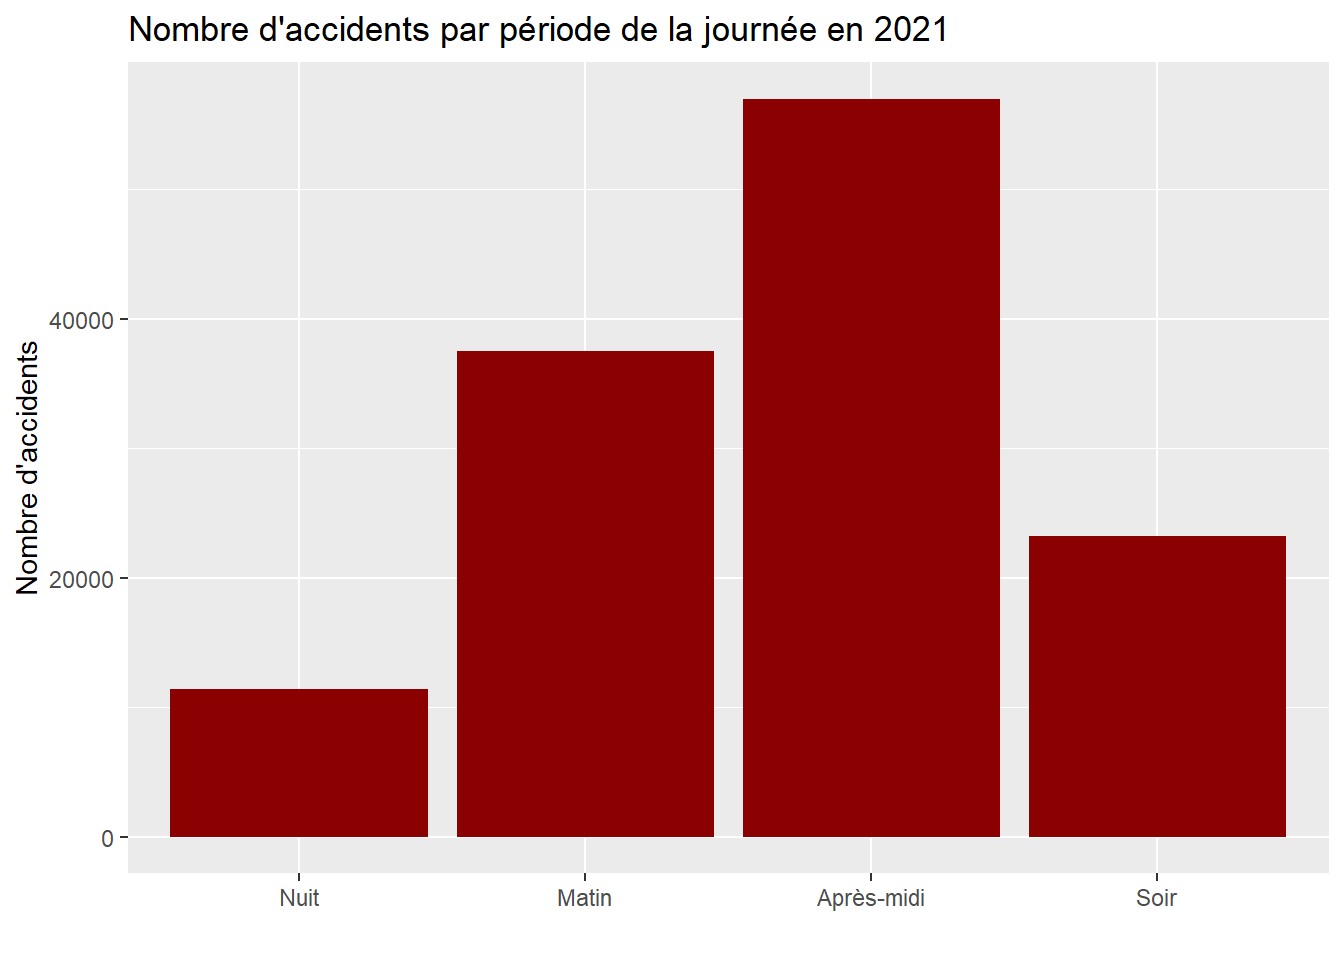
\includegraphics{FLAL_stats_files/figure-latex/unnamed-chunk-2-1.pdf}

\hypertarget{est-ce-que-les-usagers-influencent-la-gravituxe9-des-accidents}{%
\section{Est ce que les usagers influencent la gravité des accidents
?}\label{est-ce-que-les-usagers-influencent-la-gravituxe9-des-accidents}}

\hypertarget{commenuxe7ons-par-uxe9tudier-si-luxe2ge-du-conducteur-est-en-corruxe9lation-avec-la-gravituxe9-de-laccident}{%
\subsection{Commençons par étudier si l'âge du conducteur est en
corrélation avec la gravité de
l'accident}\label{commenuxe7ons-par-uxe9tudier-si-luxe2ge-du-conducteur-est-en-corruxe9lation-avec-la-gravituxe9-de-laccident}}

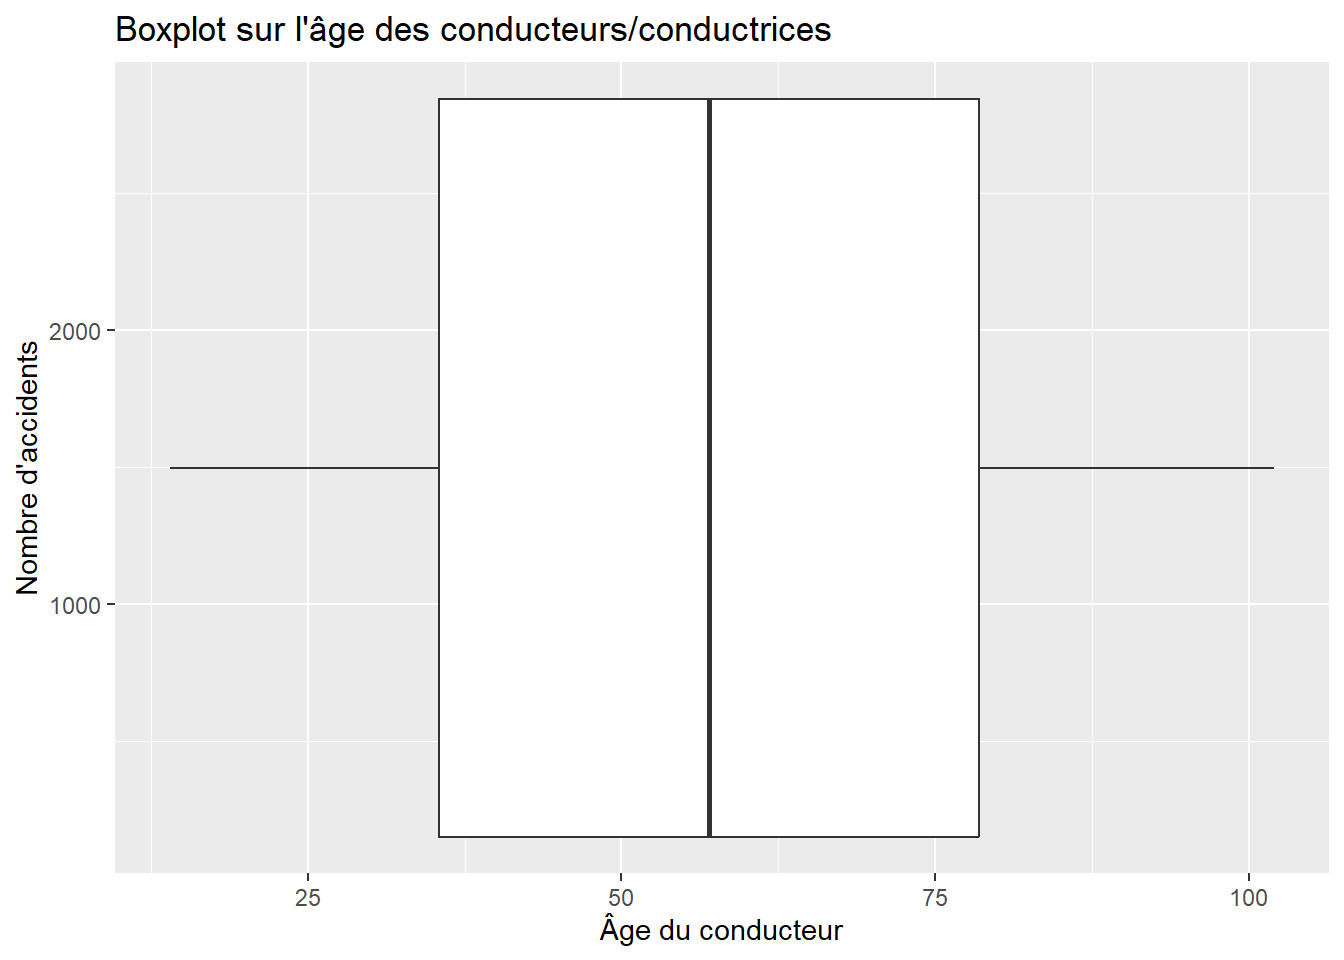
\includegraphics{FLAL_stats_files/figure-latex/unnamed-chunk-3-1.pdf}

\begin{verbatim}
## $stats
## [1]  14.0  35.5  57.0  78.5 102.0
## 
## $n
## [1] 87
## 
## $conf
## [1] 49.71607 64.28393
## 
## $out
## numeric(0)
\end{verbatim}

Sur 126086 accidents de la route en 2021, 50 \% des conducteurs ont
moins de 57 ans. 50 \% d'entre eux ont entre 35.5 et 78.5 ans.

Dans ce cas, l'intervalle de confiance est {[}49.7,64.3{]}, ce qui
signifie que l'on peut être raisonnablement sûr que la moyenne de l'âge
dans la population dont l'échantillon a été prélevé se trouve dans cette
plage avec une probabilité de 95\%.

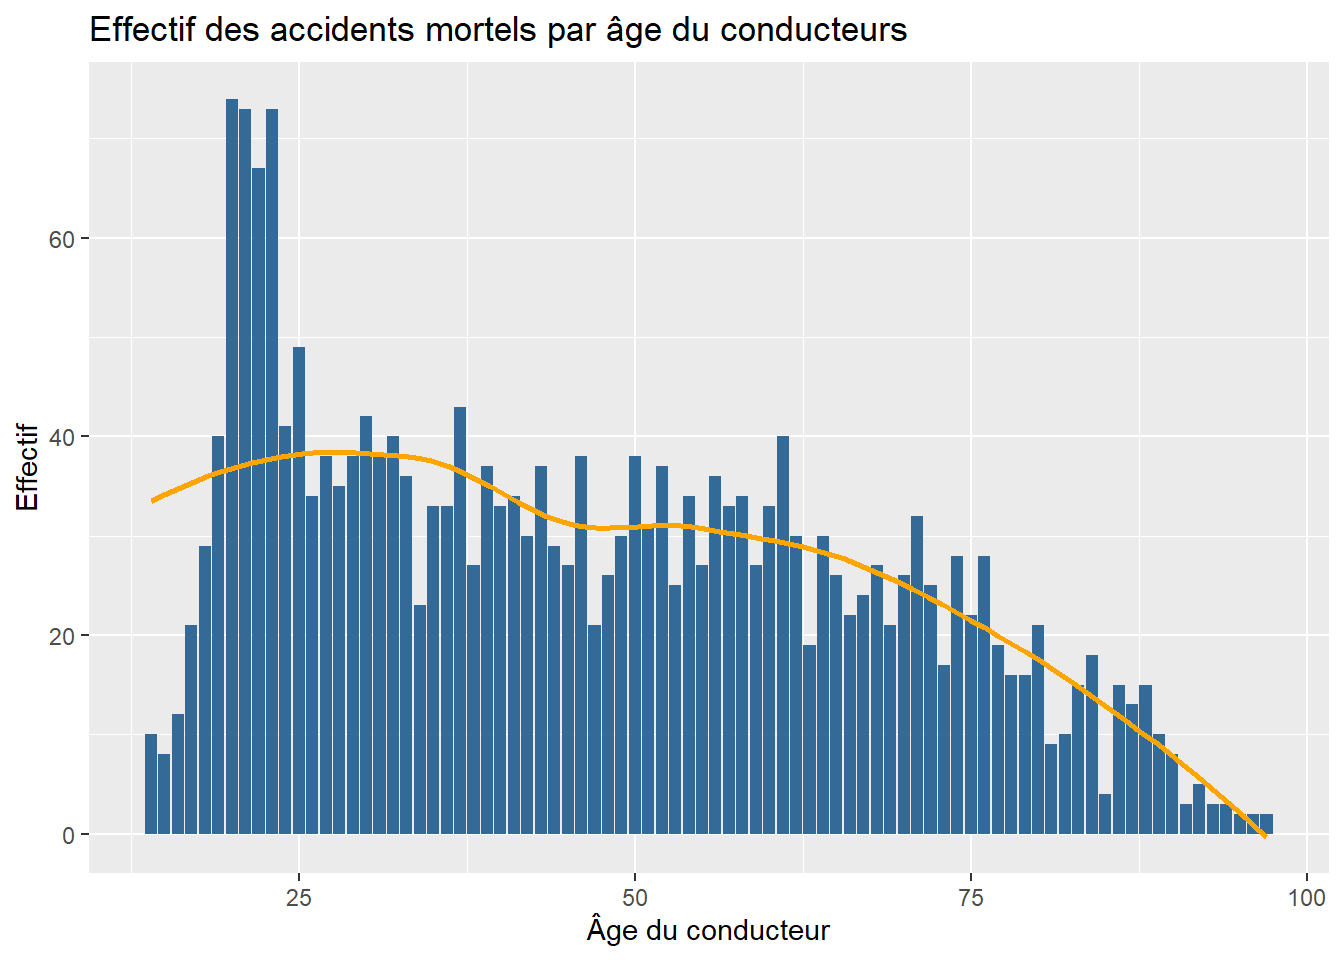
\includegraphics{FLAL_stats_files/figure-latex/unnamed-chunk-4-1.pdf}
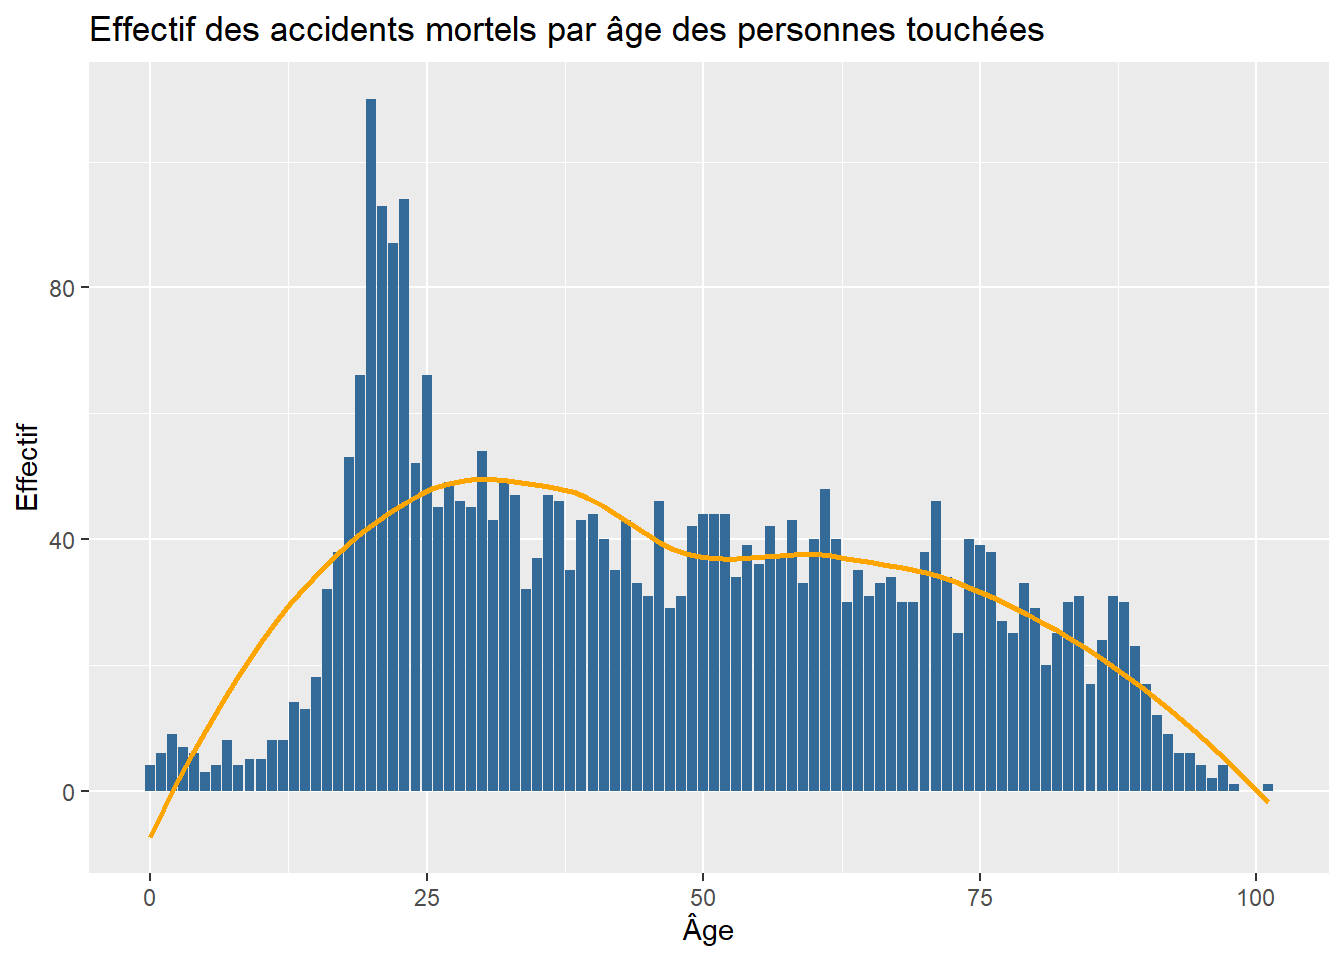
\includegraphics{FLAL_stats_files/figure-latex/unnamed-chunk-4-2.pdf}

On constate la même croissance du nombre d'accidents mortels (conducteur
ou non) de 0 à 23 ans, les personnes touchées sont plus nombreuses, ce
qui est normal il y a les passagers ajoutés. La tendance décroît
fortement de 23 à 40 ans avant de rester plus ou moins au même niveau
jusqu'à environ 70 ans. Pour les conducteurs, ont constate une
décroissance nette plus tôt que chez les personnes touchées, une
hypothèse serait que plus l'âge augmente, moins il y a de conducteurs.

Le fort pique autour de 20 ans pourrait s'expliquer par l'âge de
l'obtention du permis de conduire qui se traduit par un manque
d'expérience en tant que conducteur.

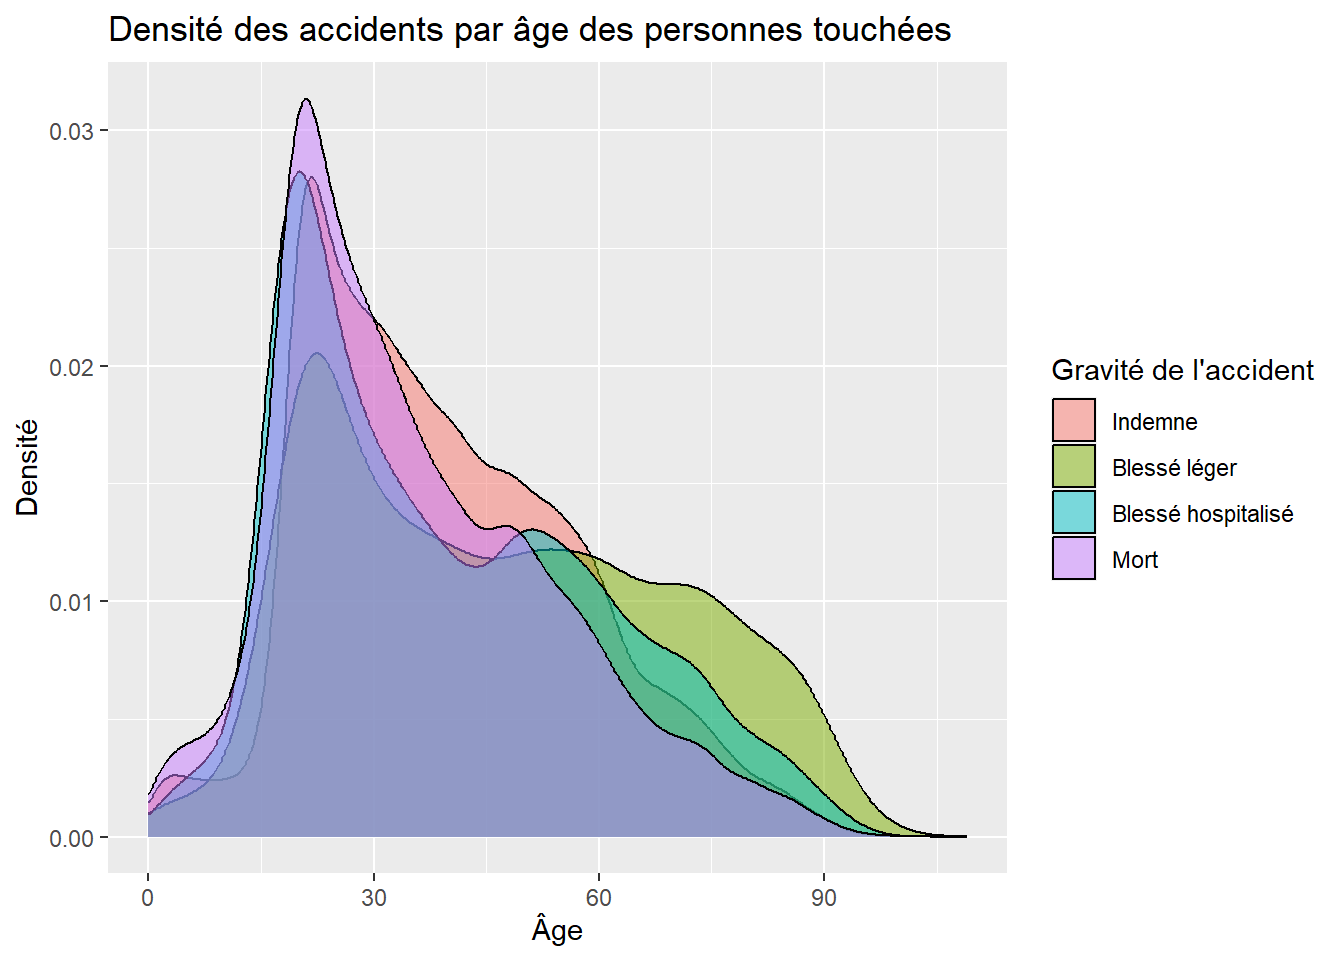
\includegraphics{FLAL_stats_files/figure-latex/unnamed-chunk-5-1.pdf}

De manière générale, le graphique de densité montre comment les
distributions de l'âge des conducteurs diffèrent selon la gravité de
l'accident. On remarque un fort pic de densité autour de 20 ans ce qui
laisse penser à une forte corrélation entre l'age et la gravité de
l'accident.

\begin{verbatim}
## 
## Call:
## glm(formula = grav_bin ~ age, family = binomial(), data = sub_df)
## 
## Deviance Residuals: 
##     Min       1Q   Median       3Q      Max  
## -1.4426  -1.3180   0.9822   1.0296   1.2298  
## 
## Coefficients:
##               Estimate Std. Error z value Pr(>|z|)    
## (Intercept)  0.6048416  0.0129956   46.54   <2e-16 ***
## age         -0.0066719  0.0003048  -21.89   <2e-16 ***
## ---
## Signif. codes:  0 '***' 0.001 '**' 0.01 '*' 0.05 '.' 0.1 ' ' 1
## 
## (Dispersion parameter for binomial family taken to be 1)
## 
##     Null deviance: 170975  on 126085  degrees of freedom
## Residual deviance: 170495  on 126084  degrees of freedom
## AIC: 170499
## 
## Number of Fisher Scoring iterations: 4
\end{verbatim}

Les résultats de la régression logistique indiquent que l'âge est
significativement associé à la gravité des accidents. Plus précisément,
pour une unité d'augmentation de l'âge, la log-odds d'avoir une gravité
plus élevée diminue de 0,00667. Cela peut être interprété comme une
diminution de la probabilité d'avoir une gravité plus élevée pour chaque
année supplémentaire.

Le rapport des deviances (null deviance et residual deviance) montre que
le modèle ajuste bien les données, car il y a une réduction
significative de la deviance résiduelle par rapport à la deviance nulle.
En outre, l'AIC est relativement faible, ce qui indique que le modèle
est un ajustement approprié pour les données.

Le test de significativité indique que la relation entre l'âge et la
gravité de l'accident est très significative (p-value \textless{}
2e-16), ce qui renforce l'idée que l'âge est un facteur important à
prendre en compte dans l'évaluation de la gravité des accidents de la
route.

En résumé, les résultats de la régression logistique soutiennent l'idée
que l'âge est significativement associé à la gravité des accidents de la
route et que le modèle est un ajustement approprié pour les données.

\hypertarget{est-ce-que-le-sexe-influence-la-gravituxe9-des-accidents}{%
\section{Est-ce que le sexe influence la gravité des accidents
?}\label{est-ce-que-le-sexe-influence-la-gravituxe9-des-accidents}}

\begin{Shaded}
\begin{Highlighting}[]
\NormalTok{sub\_df }\OtherTok{\textless{}{-}}\NormalTok{ df[, }\FunctionTok{c}\NormalTok{(}\StringTok{"grav"}\NormalTok{, }\StringTok{"sexe"}\NormalTok{)]}

\CommentTok{\# enleve les na}
\NormalTok{sub\_df }\OtherTok{\textless{}{-}} \FunctionTok{na.omit}\NormalTok{(sub\_df) }\SpecialCharTok{\%\textgreater{}\%} \FunctionTok{filter}\NormalTok{(sexe }\SpecialCharTok{!=} \SpecialCharTok{{-}}\DecValTok{1}\NormalTok{)}

\NormalTok{tab }\OtherTok{\textless{}{-}} \FunctionTok{table}\NormalTok{(sub\_df}\SpecialCharTok{$}\NormalTok{sexe, sub\_df}\SpecialCharTok{$}\NormalTok{grav)}

\CommentTok{\# Conversion de la table croisée en un data frame}
\NormalTok{df\_s }\OtherTok{\textless{}{-}} \FunctionTok{as.data.frame.matrix}\NormalTok{(tab)}
\NormalTok{df\_s}\SpecialCharTok{$}\NormalTok{sexe }\OtherTok{\textless{}{-}} \FunctionTok{rownames}\NormalTok{(df\_s)}

\CommentTok{\# Mise en forme des données pour un diagramme en barres empilées}
\NormalTok{df\_long }\OtherTok{\textless{}{-}}\NormalTok{ tidyr}\SpecialCharTok{::}\FunctionTok{gather}\NormalTok{(df\_s, }\AttributeTok{key =} \StringTok{"grav"}\NormalTok{, }\AttributeTok{value =} \StringTok{"count"}\NormalTok{, }\SpecialCharTok{{-}}\NormalTok{sexe)}
\NormalTok{df\_long}\SpecialCharTok{$}\NormalTok{grav }\OtherTok{\textless{}{-}} \FunctionTok{factor}\NormalTok{(df\_long}\SpecialCharTok{$}\NormalTok{grav, }\AttributeTok{levels =} \FunctionTok{c}\NormalTok{(}\StringTok{"1"}\NormalTok{, }\StringTok{"2"}\NormalTok{, }\StringTok{"3"}\NormalTok{, }\StringTok{"4"}\NormalTok{))}
\NormalTok{df\_long}\SpecialCharTok{$}\NormalTok{sexe }\OtherTok{\textless{}{-}} \FunctionTok{factor}\NormalTok{(df\_long}\SpecialCharTok{$}\NormalTok{sexe, }\AttributeTok{levels =} \FunctionTok{c}\NormalTok{(}\StringTok{"1"}\NormalTok{, }\StringTok{"2"}\NormalTok{))}

\CommentTok{\# Convertir la variable grav en factor avec les niveaux correspondants}
\NormalTok{df\_long}\SpecialCharTok{$}\NormalTok{grav }\OtherTok{\textless{}{-}} \FunctionTok{factor}\NormalTok{(df\_long}\SpecialCharTok{$}\NormalTok{grav, }\AttributeTok{levels =} \DecValTok{1}\SpecialCharTok{:}\DecValTok{4}\NormalTok{,}
                       \AttributeTok{labels =} \FunctionTok{c}\NormalTok{(}\StringTok{"Indemne"}\NormalTok{, }\StringTok{"Mort"}\NormalTok{, }\StringTok{"Blessé hospitalisé"}\NormalTok{, }\StringTok{"Blessé léger"}\NormalTok{))}

\NormalTok{df\_long}\SpecialCharTok{$}\NormalTok{sexe }\OtherTok{\textless{}{-}} \FunctionTok{factor}\NormalTok{(df\_long}\SpecialCharTok{$}\NormalTok{sexe, }\AttributeTok{levels =} \DecValTok{1}\SpecialCharTok{:}\DecValTok{2}\NormalTok{,}
                       \AttributeTok{labels =} \FunctionTok{c}\NormalTok{(}\StringTok{"Homme"}\NormalTok{, }\StringTok{"Femme"}\NormalTok{))}

\CommentTok{\# Définir les couleurs personnalisées}
\NormalTok{colors }\OtherTok{\textless{}{-}} \FunctionTok{c}\NormalTok{(}\StringTok{"Homme"} \OtherTok{=} \StringTok{"pink"}\NormalTok{, }
            \StringTok{"Femme"} \OtherTok{=} \StringTok{"lightblue"}\NormalTok{)}


\CommentTok{\# Réorganiser les niveaux de la variable "grav" en fonction de la fréquence}
\NormalTok{df\_long}\SpecialCharTok{$}\NormalTok{grav }\OtherTok{\textless{}{-}} \FunctionTok{reorder}\NormalTok{(df\_long}\SpecialCharTok{$}\NormalTok{grav, }\FunctionTok{desc}\NormalTok{(df\_long}\SpecialCharTok{$}\NormalTok{count))}

\CommentTok{\# Créer le graphique}
\FunctionTok{ggplot}\NormalTok{(df\_long, }\FunctionTok{aes}\NormalTok{(}\AttributeTok{x =}\NormalTok{ grav, }\AttributeTok{fill =}\NormalTok{ sexe)) }\SpecialCharTok{+}
  \FunctionTok{geom\_col}\NormalTok{(}\AttributeTok{position =} \StringTok{"dodge"}\NormalTok{, }\FunctionTok{aes}\NormalTok{(}\AttributeTok{y =}\NormalTok{ count)) }\SpecialCharTok{+}
  \FunctionTok{scale\_fill\_manual}\NormalTok{(}\AttributeTok{values =}\NormalTok{ colors, }\AttributeTok{name =} \StringTok{"Sexe"}\NormalTok{,}
                    \AttributeTok{labels =} \FunctionTok{c}\NormalTok{(}\StringTok{"Homme"}\NormalTok{, }\StringTok{"Femme"}\NormalTok{)) }\SpecialCharTok{+}
  \FunctionTok{labs}\NormalTok{(}\AttributeTok{title =} \StringTok{"Gravité des accidents par sexe"}\NormalTok{, }\AttributeTok{x =} \StringTok{""}\NormalTok{, }\AttributeTok{y =} \StringTok{"Nombre d\textquotesingle{}accidents"}\NormalTok{) }\SpecialCharTok{+} \FunctionTok{theme\_gray}\NormalTok{()}
\end{Highlighting}
\end{Shaded}

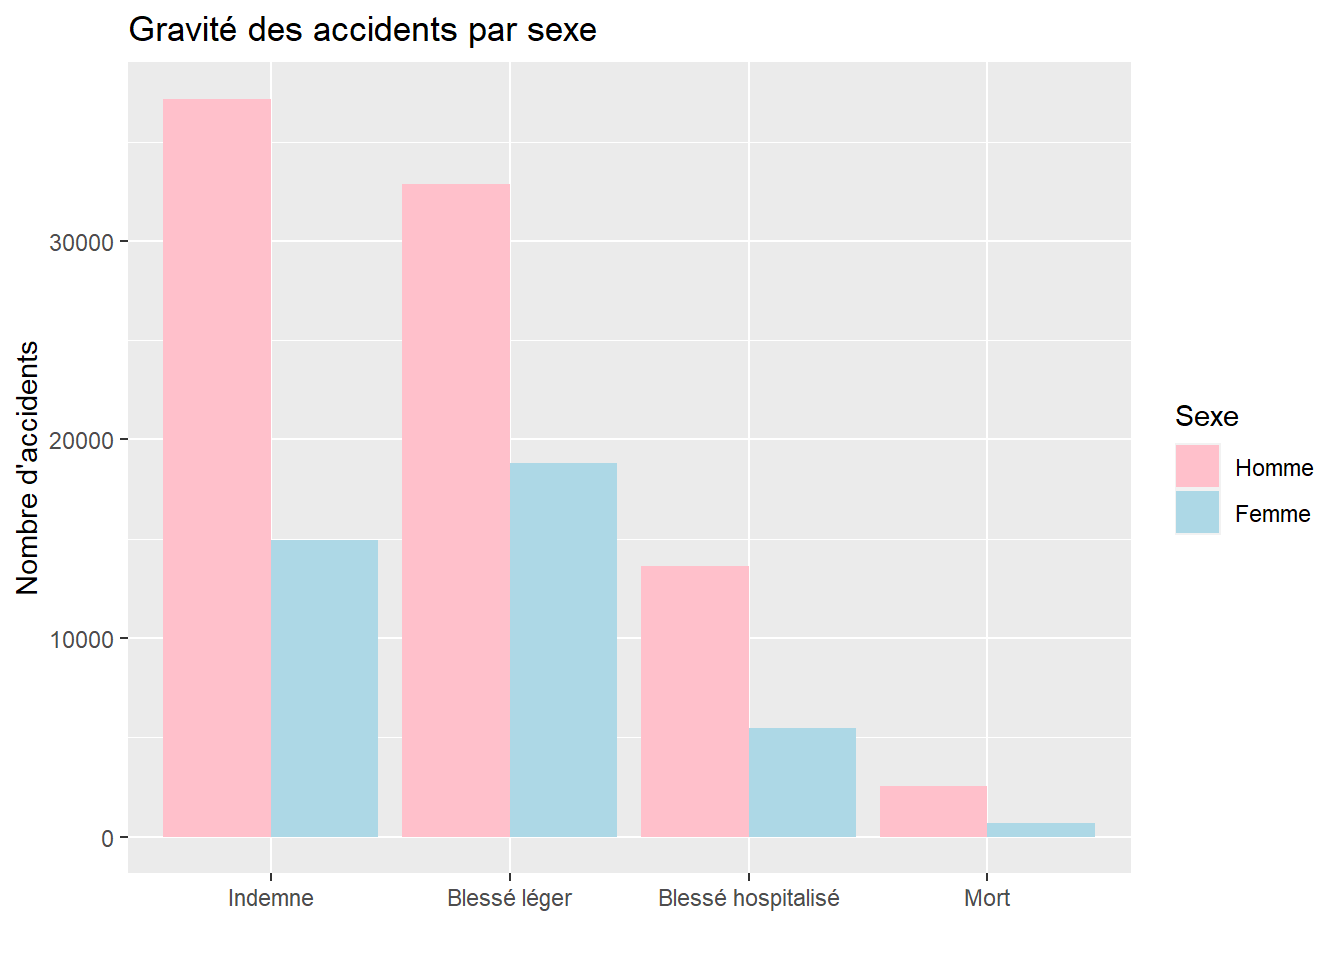
\includegraphics{FLAL_stats_files/figure-latex/unnamed-chunk-7-1.pdf}
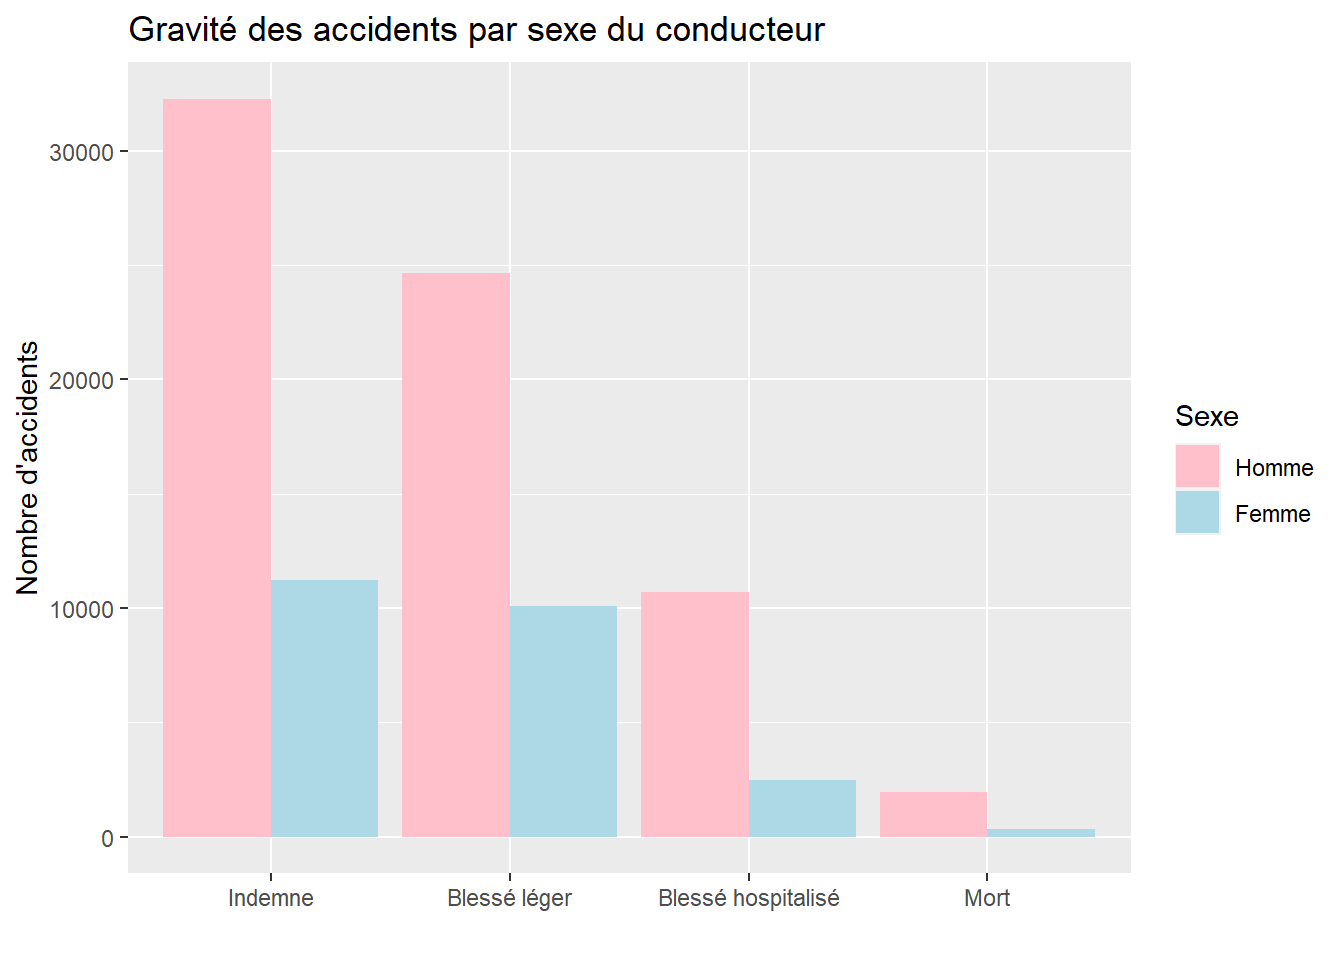
\includegraphics{FLAL_stats_files/figure-latex/unnamed-chunk-8-1.pdf}

On remarque que, conducteur/trice ou non, la tendance reste la même au
niveau de la gravité. La quantité d'accidents reste plus importe chez
les hommes que chez les femmes.

\begin{verbatim}
## 
##  Pearson's Chi-squared test
## 
## data:  table(df_conducteurs$sexe, df_conducteurs$grav)
## X-squared = 686.69, df = 6, p-value < 2.2e-16
\end{verbatim}

Puisque la p-value est inférieure au seuil de significativité
communément utilisé de 0,05, on peut rejeter l'hypothèse nulle selon
laquelle il n'y a pas d'association entre le sexe et la gravité des
accidents de la route. On peut donc conclure qu'il y a une association
significative entre le sexe et la gravité des accidents de la route en
France en 2021.

Cela signifie que le sexe des conducteurs est statistiquement
significatif pour prédire la gravité des accidents de la route en France
en 2021. Cependant, il est important de noter que les résultats de ce
test ne permettent pas de déterminer la direction de l'association
(c'est-à-dire, si les accidents graves sont plus fréquents chez les
hommes ou chez les femmes).

\hypertarget{est-ce-que-le-lieu-influence-la-gravituxe9-des-accidents}{%
\subsection{Est ce que le lieu influence la gravité des accidents
?}\label{est-ce-que-le-lieu-influence-la-gravituxe9-des-accidents}}

\begin{verbatim}
## Reading layer `regions-version-simplifiee' from data source 
##   `https://raw.githubusercontent.com/gregoiredavid/france-geojson/master/regions-version-simplifiee.geojson' 
##   using driver `GeoJSON'
## Simple feature collection with 13 features and 2 fields
## Geometry type: MULTIPOLYGON
## Dimension:     XY
## Bounding box:  xmin: -5.103601 ymin: 41.36705 xmax: 9.559721 ymax: 51.0884
## Geodetic CRS:  WGS 84
\end{verbatim}

\includegraphics{FLAL_stats_files/figure-latex/unnamed-chunk-10-1.pdf}
\includegraphics{FLAL_stats_files/figure-latex/unnamed-chunk-10-2.pdf}

\begin{verbatim}
## 
##  Pearson's Chi-squared test
## 
## data:  cont_table
## X-squared = 6065.5, df = 39, p-value < 2.2e-16
\end{verbatim}

Le résultat du test montre une statistique de test de 6065.5 et un degré
de liberté de 39, ce qui donne une p-value inférieure à 2.2e-16.

La p-value est très faible, ce qui suggère qu'il y a une forte
association entre la région et la gravité de l'accident. Autrement dit,
la gravité des accidents semble varier significativement selon la région
où ils se produisent.

\begin{verbatim}
## Reading layer `departements' from data source 
##   `https://france-geojson.gregoiredavid.fr/repo/departements.geojson' 
##   using driver `GeoJSON'
## Simple feature collection with 96 features and 2 fields
## Geometry type: MULTIPOLYGON
## Dimension:     XY
## Bounding box:  xmin: -5.138001 ymin: 41.36216 xmax: 9.559226 ymax: 51.08854
## Geodetic CRS:  WGS 84
\end{verbatim}

\includegraphics{FLAL_stats_files/figure-latex/unnamed-chunk-11-1.pdf}
\includegraphics{FLAL_stats_files/figure-latex/unnamed-chunk-11-2.pdf}

\begin{verbatim}
## 
##  Pearson's Chi-squared test
## 
## data:  cont_table
## X-squared = 10960, df = 318, p-value < 2.2e-16
\end{verbatim}

Dans les deux résultats, la statistique de test est très élevée (6065.5
pour les régions et 10960 pour les départements), ce qui suggère qu'il
existe un lien significatif entre la région/departement et la gravité de
l'accident.

\hypertarget{est-ce-que-lenvironnement-influence-la-gravituxe9-des-accidents}{%
\subsection{Est ce que l'environnement influence la gravité des
accidents
?}\label{est-ce-que-lenvironnement-influence-la-gravituxe9-des-accidents}}

\hypertarget{est-ce-que-la-catuxe9gorie-de-vuxe9hicule-influence-la-gravituxe9}{%
\subsubsection{Est ce que la catégorie de véhicule influence la gravité
?}\label{est-ce-que-la-catuxe9gorie-de-vuxe9hicule-influence-la-gravituxe9}}

\includegraphics{FLAL_stats_files/figure-latex/unnamed-chunk-12-1.pdf}

\begin{verbatim}
## 
## Call:
## glm(formula = grav_binary ~ categorie, family = binomial, data = df)
## 
## Deviance Residuals: 
##     Min       1Q   Median       3Q      Max  
## -0.8727  -0.5807  -0.5807  -0.4624   2.3695  
## 
## Coefficients:
##                               Estimate Std. Error  z value Pr(>|z|)    
## (Intercept)                  -1.694609   0.008903 -190.339  < 2e-16 ***
## categorieCamion              -0.487282   0.060194   -8.095 5.72e-16 ***
## categorieDeux-roues           0.925468   0.017959   51.533  < 2e-16 ***
## categorieEngin spécial        0.184850   0.125430    1.474    0.141    
## categorieTransport en commun -1.050340   0.106775   -9.837  < 2e-16 ***
## categorieVoiture             -0.513298   0.036831  -13.937  < 2e-16 ***
## ---
## Signif. codes:  0 '***' 0.001 '**' 0.01 '*' 0.05 '.' 0.1 ' ' 1
## 
## (Dispersion parameter for binomial family taken to be 1)
## 
##     Null deviance: 118832  on 129092  degrees of freedom
## Residual deviance: 115606  on 129087  degrees of freedom
## AIC: 115618
## 
## Number of Fisher Scoring iterations: 5
\end{verbatim}

La première partie de la sortie donne quelques informations sur la
qualité de l'ajustement du modèle, notamment les résidus de deviance.
Dans l'ensemble, les résidus semblent assez faibles, ce qui suggère que
le modèle s'adapte bien aux données.

La deuxième partie de la sortie présente les coefficients estimés pour
chaque niveau de la variable explicative (les différentes catégories de
véhicules). Les coefficients indiquent l'effet de chaque niveau de la
variable explicative sur la probabilité de gravité de l'accident. Par
exemple, la variable categorieTransport en commun a un coefficient
négatif (-1.050340), ce qui signifie qu'être impliqué dans un accident
avec un transport en commun diminue la probabilité de gravité de
l'accident par rapport aux autres catégories de véhicules.

En somme, ces résultats indiquent que la catégorie de véhicule est un
facteur significatif pour prédire la gravité de l'accident, et que
certains types de véhicules ont une probabilité de gravité plus élevée
ou plus faible que d'autres.

\hypertarget{est-ce-que-luxe9quipement-de-suxe9curituxe9-influence-la-gravituxe9}{%
\subsubsection{Est ce que l'équipement de sécurité influence la gravité
?}\label{est-ce-que-luxe9quipement-de-suxe9curituxe9-influence-la-gravituxe9}}

\includegraphics{FLAL_stats_files/figure-latex/unnamed-chunk-13-1.pdf}

\begin{itemize}
\item
  Pour les véhicules :

\begin{verbatim}
- On regarde la gravité en fonction de la sécurité installée pour l'usager (ceinture airbag pour les voitures, casque gant veste pour les motards)
\end{verbatim}
\item
  Pour l'environnement : - On regarde la gravité en fonction de la
  vitesse autorisée (en agglo (50km/h)n etc\ldots) - On regarde le nb et
  la gravité en fonction de l'état de la route (mouillée, eneigée,
  sèche) - On regarde le nb et la gravité en fonction de l'éclairage de
  la route (nuit noire, jour, éclairage urbain etc\ldots)
\end{itemize}

\includegraphics{FLAL_stats_files/figure-latex/unnamed-chunk-14-1.pdf}

\end{document}
